\section{Results and Analysis}
\label{sec:results-analysis}

This section presents the experimental evidence in the same order in which the benchmark design was developed and validated. The first phase establishes the baseline behavior of the benchmark and verifies the methodological assumptions needed for fair comparison. The second phase provides the main matched grid-level timing evidence across the selected PyTorch CUDA accumulation paths. The third phase complements the timing results with profiler evidence for representative cases, allowing the observed performance differences to be related to the CUDA execution paths used by each API.

The analysis therefore separates three roles. Phase 1 is treated as a calibration and validation phase, because its purpose is to justify the final benchmark protocol rather than to provide the main paper-level performance claim. Phase 2 is treated as the primary timing phase, because it compares the selected operations across a matched workload grid. Phase 3 is treated as the attribution phase, because it explains selected Phase 2 patterns through CUDA profiler evidence. This separation is important because the study does not rely on a single timing table or a single profiler run; instead, the final interpretation combines protocol validation, matched timing, and representative execution-path analysis.

\subsection{Phase 1 Baseline Calibration and Methodological Checks}

Phase~1 calibrated the final benchmark protocol rather than supporting paper-level performance claims. Preliminary runs established a dense-gradient accumulation scope that includes output allocation or zero initialization where required by the operation design. They also confirmed that \texttt{Embedding.\allowbreak backward} should be treated as a standard framework path with its own dispatch behavior, rather than a syntactic alias for the direct accumulation APIs.

The calibration phase fixed the acceptance and interpretation rules used later. Tolerance-based correctness validation precedes acceptance of timing rows because repeated indices and different CUDA paths can change floating-point accumulation order. Median CUDA-event latency summarizes each timing distribution; a winner is decisive only when the runner-up is more than 5\% slower. Smaller differences remain practical ties.

Phase~1 also motivated varying uniform, Zipf, and hotspot-style index distributions alongside workload shape. The final protocol combines matched workloads, correctness-gated rows, median timing, and practical-margin classification, while separating grid-level timing evidence from profiler-based attribution. The main performance evidence begins with Phase~2.

\subsection{Matched Phase 2 Benchmark Results}

The matched Phase 2 benchmark provides the main grid-level evidence for the study. In this phase, the three selected PyTorch accumulation paths were compared under shared workload configurations, using the same rows, index counts, feature dimensions, distribution types, layout settings, and cache conditions within each matched case. The purpose of this phase was to determine whether the fastest API path is stable across environments or whether it changes with the workload and software/hardware stack.

Table~\ref{tab:phase2-winner-counts} summarizes the practical-margin winner counts across the matched Phase 2 grid. The GTX1650Ti stack favored \texttt{embedding} most often, with 96 decisive wins out of 162 matched configurations. The same environment selected \texttt{index\_\allowbreak add} in 60 configurations, while \texttt{scatter\_\allowbreak add} did not obtain a decisive win under the practical-margin rule. Six configurations were classified as ties. In contrast, the T4 stack favored \texttt{scatter\_\allowbreak add} most often, with 92 decisive wins out of 162 configurations. The repeated T4 run reproduced the same qualitative pattern, with \texttt{scatter\_\allowbreak add} selected in 93 out of 162 configurations.

% Source summary: sparse-gradient/phase2_analysis_v2/ and matched Phase 2 analysis.
\begin{table*}[t]
\centering
\fontsize{9}{11}\selectfont
\caption{Matched Phase 2 winner counts for the three primary accumulation paths under the 5\% practical-margin rule.}
\label{tab:phase2-winner-counts}
\setlength{\tabcolsep}{3pt}
\renewcommand{\arraystretch}{1.12}
\begin{tabularx}{\linewidth}{@{}lrrrr>{\raggedright\arraybackslash}X>{\raggedright\arraybackslash}X@{}}
\toprule
Environment & \texttt{index\_add} & \texttt{scatter\_add} & \texttt{embedding} & Tie & Total matched configurations & Most frequent decisive API \\
\midrule
GTX1650Ti & 60 & 0 & 96 & 6 & 162 & \texttt{embedding} \\
T4 & 5 & 92 & 25 & 40 & 162 & \texttt{scatter\_add} \\
T4\_repeat & 1 & 93 & 27 & 41 & 162 & \texttt{scatter\_add} \\
\bottomrule
\end{tabularx}
\end{table*}


The Phase~2 results show a change in the most frequently favored path across the measured stacks. The GTX1650Ti stack most often favors the embedding backward path, whereas the T4 stack and its repeat run most often favor the scatter-add path. This difference is not interpreted as an isolated GPU-hardware effect, because the environments differ in GPU model, operating system, PyTorch version, CUDA version, and hosted execution conditions. Instead, the result motivates a stack-level interpretation: the relative cost of the available PyTorch CUDA paths depends on the combination of workload structure and execution environment.

The practical-margin rule is important for interpreting these counts. Configurations in which the fastest and runner-up operations differ by no more than the selected 5\% threshold are retained as near-ties rather than treated as decisive evidence. This prevents small timing differences from being overinterpreted as meaningful API-level superiority. Consequently, the Phase 2 result should be read as a matched practical-performance characterization, not as a statistical proof of an API ordering that applies across workloads and stacks.

\subsection{Representative Phase 3 Profiling Results}

Phase 3 complements the Phase 2 timing grid by profiling a representative subset of six workload cases. The purpose of this phase is not to replace the broader timing evidence, but to inspect the CUDA execution paths associated with the selected PyTorch APIs. Each representative case is evaluated for \texttt{index\_\allowbreak add}, \texttt{scatter\_\allowbreak add}, and \texttt{Embedding.\allowbreak backward}, resulting in 18 profiled case-operation rows per environment.

The profiling outputs passed the basic execution and correctness checks in both environments. Each environment produced 18 successful case-operation rows, with no failed execution status and no correctness failures. CUDA kernel attribution was available for all 18 profiled rows in both environments. The T4 environment contained one host-overhead warning, associated with the \texttt{embedding} operation in case04; this case is therefore interpreted cautiously when making GPU-clean attribution claims.

Figure~\ref{fig:phase3-median-ms} shows the representative Phase 3 event-timing medians by case and operation. These values are useful for relating the profiled subset to the broader timing behavior, but they are not treated as a replacement for the matched Phase 2 grid. The profiled subset uses a smaller number of cases and is primarily designed for attribution rather than grid-level performance counting.

\begin{figure*}[t]
\centering
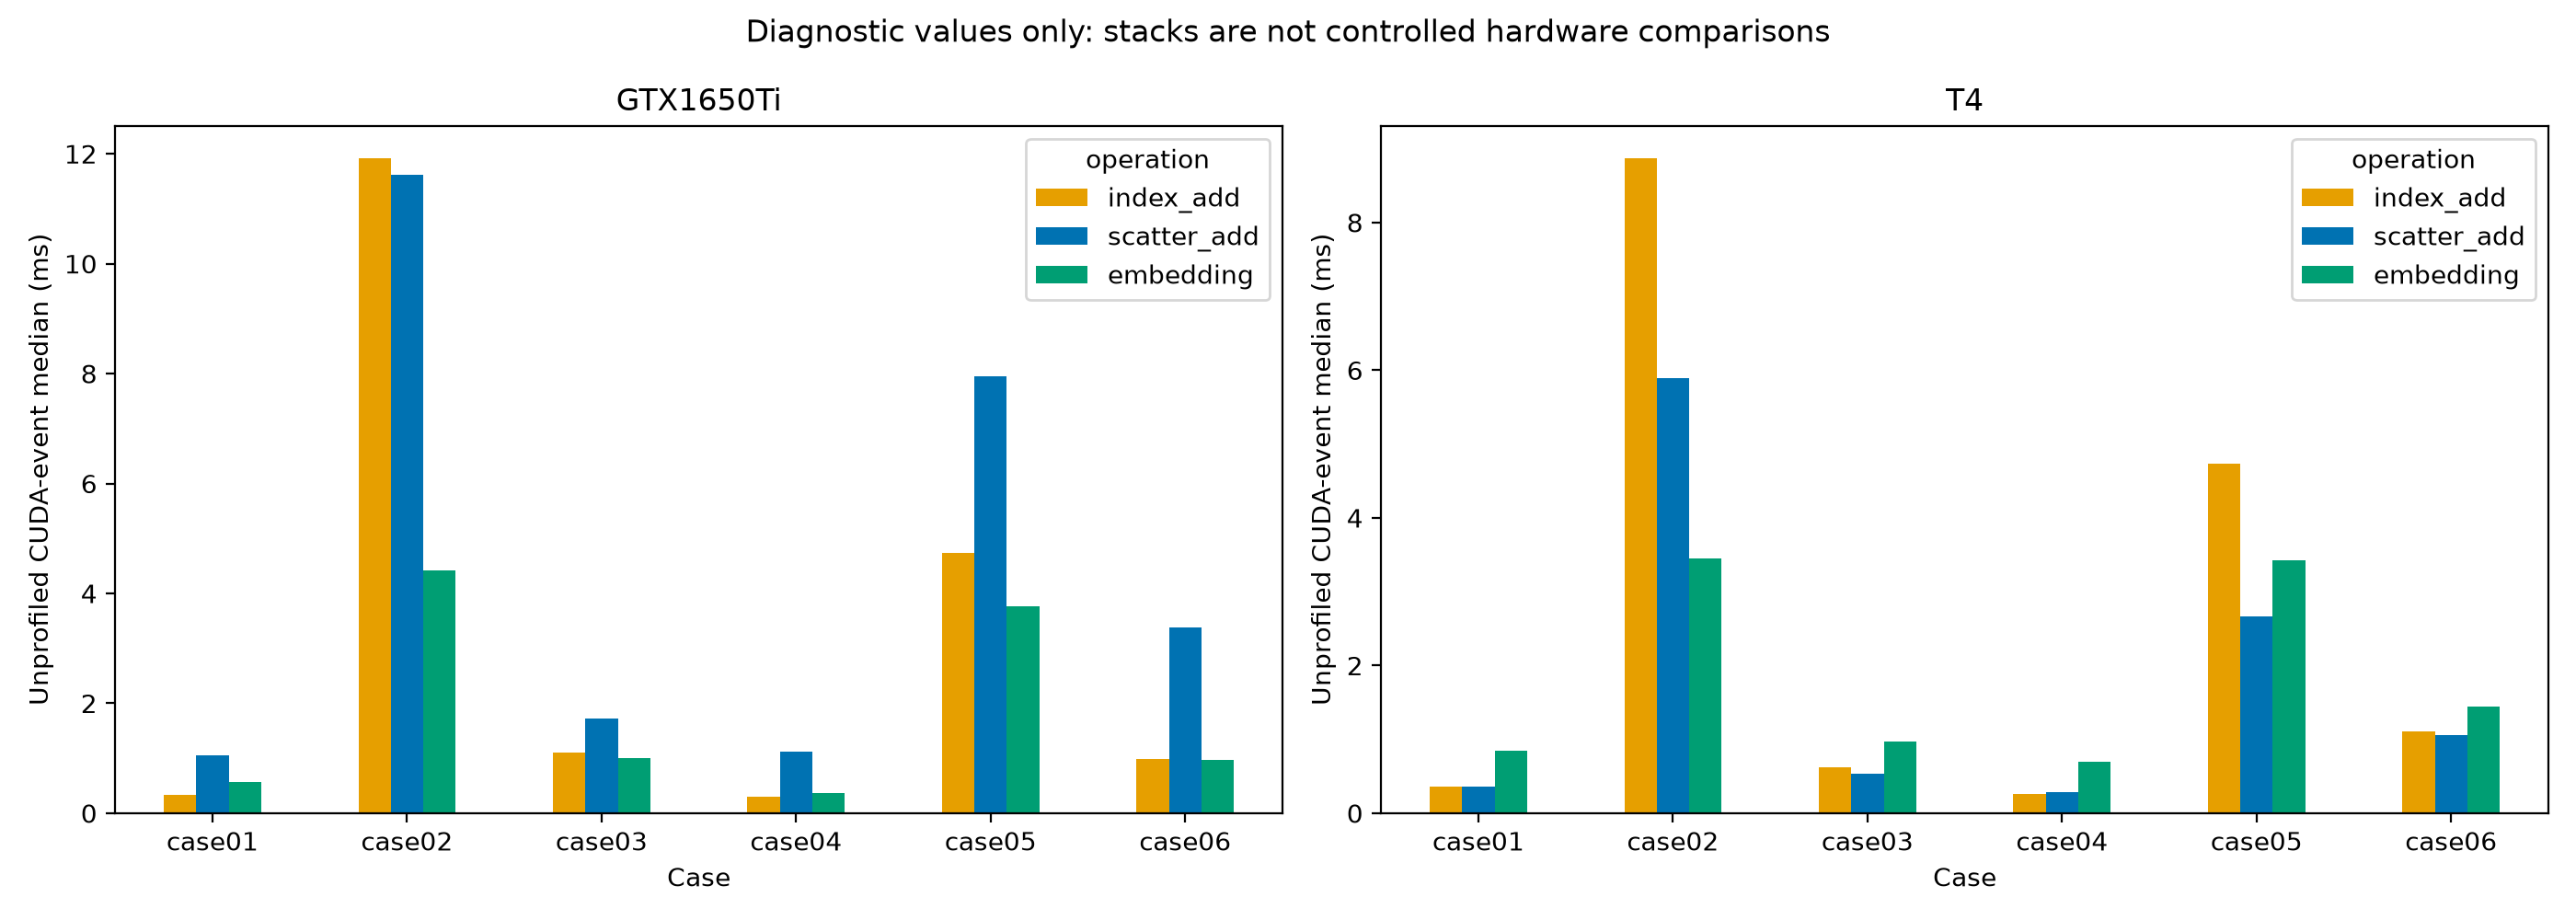
\includegraphics[width=0.95\linewidth]{figures/phase3_median_ms_by_case_operation.png}
\caption{Phase 3 median CUDA-event timing by representative case and operation. These timings describe the profiled subset and are interpreted together with the broader matched Phase 2 grid.}
\label{fig:phase3-median-ms}
\end{figure*}

Figure~\ref{fig:phase3-gpu-busy} summarizes the profiler-derived GPU-busy proxy. The proxy is used only as a warning signal for possible host overhead, not as a hardware utilization counter. Most profiled case-operation rows have high proxy values, supporting their use for execution-path attribution. The main exception is the T4 \texttt{embedding} row in case04, which is flagged and therefore not used as a clean GPU-bound claim.

\begin{figure*}[t]
\centering
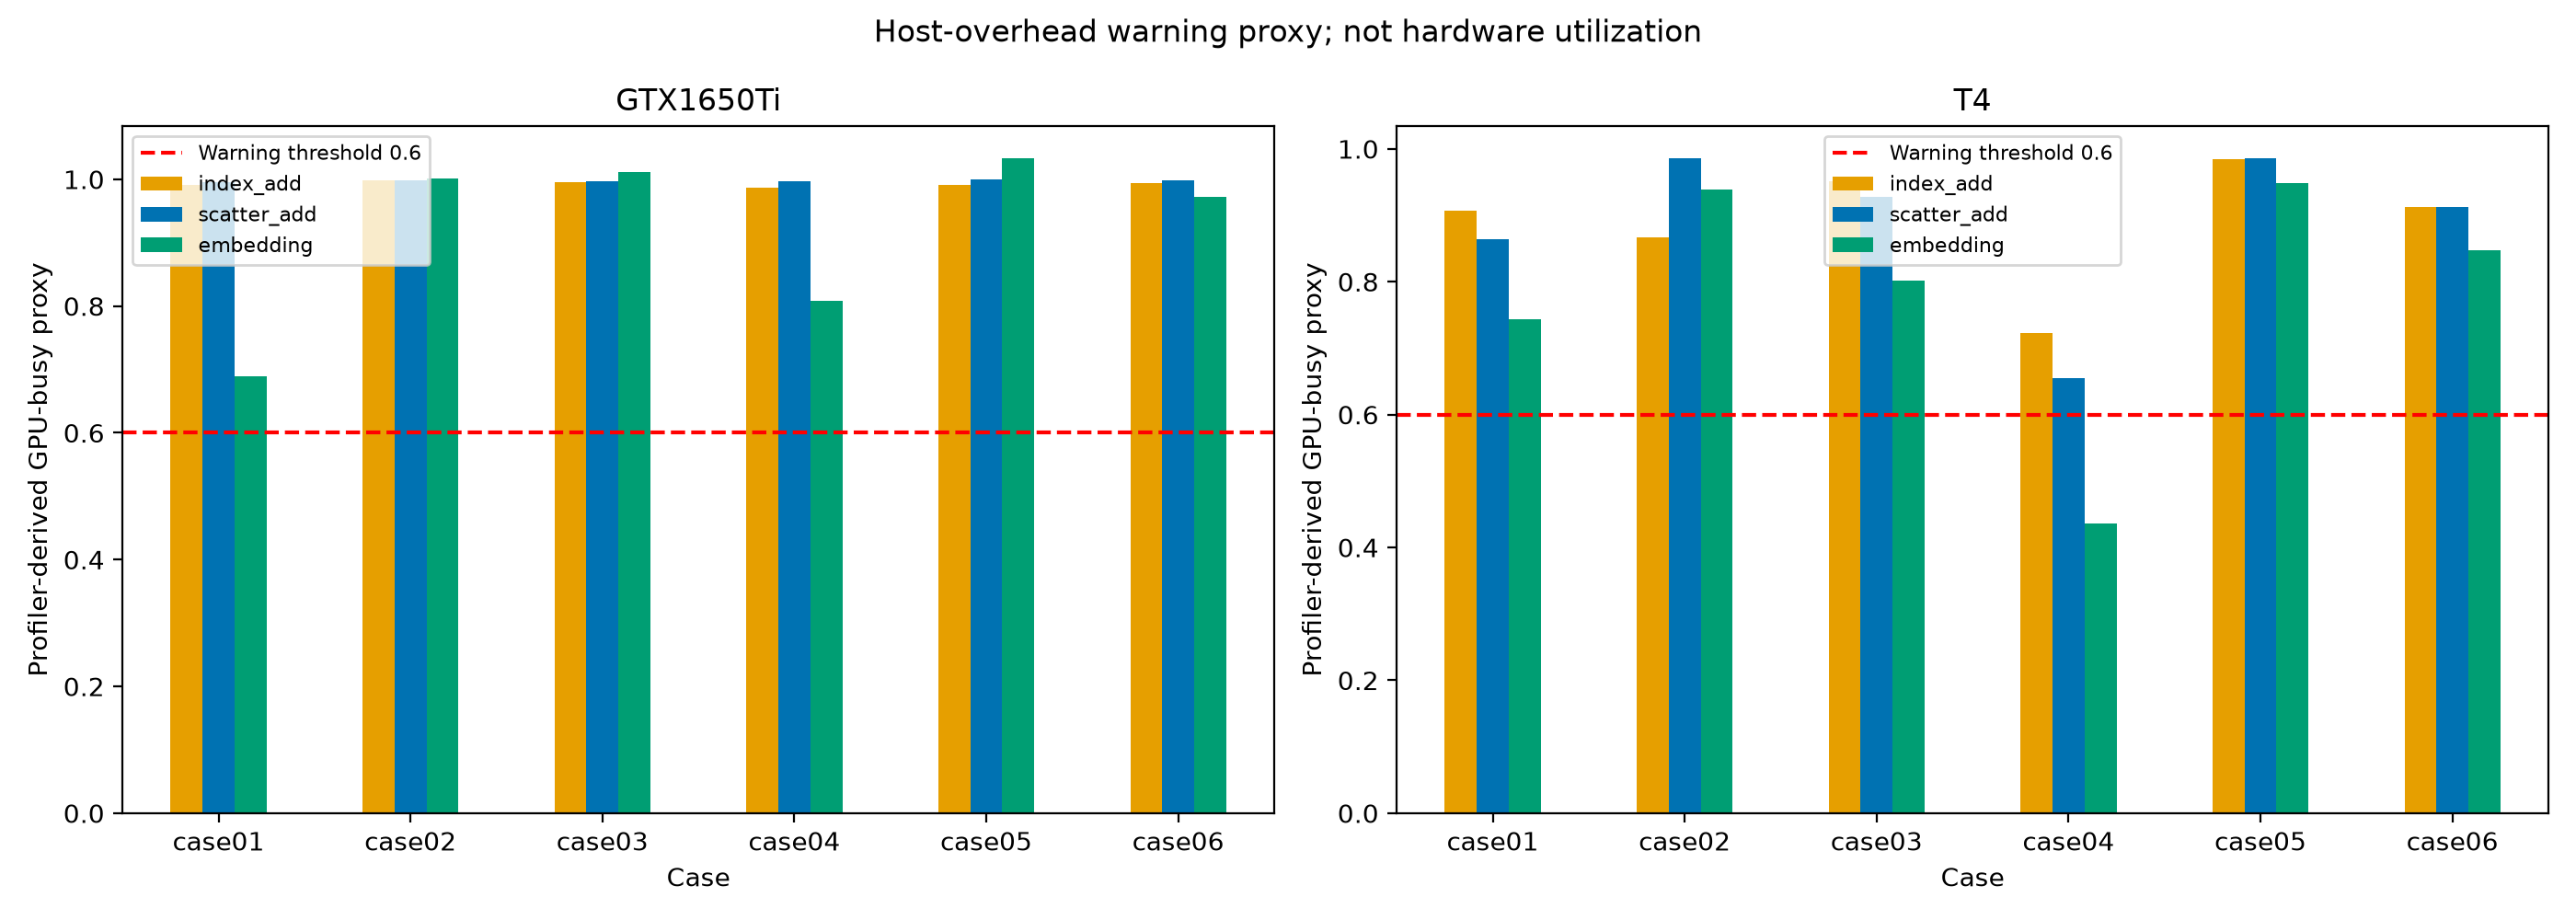
\includegraphics[width=0.95\linewidth]{figures/phase3_gpu_busy_fraction_by_case_operation.png}
\caption{Profiler-derived GPU-busy proxy by representative case and operation. The proxy is diagnostic only and is not interpreted as hardware utilization.}
\label{fig:phase3-gpu-busy}
\end{figure*}

The kernel-category summary in Table~\ref{tab:phase3-kernel-category-summary} and Figure~\ref{fig:phase3-kernel-category-share} shows that the three API paths are not merely different syntactic forms of the same CUDA behavior. The \texttt{index\_\allowbreak add} path is dominated by indexed accumulation kernels, the \texttt{scatter\_\allowbreak add} path is dominated by scatter/gather-style accumulation kernels, and the embedding backward path uses a multi-kernel composition that includes accumulation as well as sorting, scanning, or uniqueness-related components.

% Source summary: sparse-gradient/phase3_comparison_v2/phase3_kernel_category_summary.csv.
% Detailed per-case rows can be moved to an appendix or supplementary material later.
\begin{table*}[t]
\centering
\fontsize{9}{11}\selectfont
\caption{Mean CUDA kernel-category shares for the representative Phase 3 profiles. Shares are averaged across the profiled cases for each environment and operation.}
\label{tab:phase3-kernel-category-summary}
\setlength{\tabcolsep}{3pt}
\renewcommand{\arraystretch}{1.12}
\begin{tabularx}{\linewidth}{@{}l l >{\raggedright\arraybackslash}X >{\raggedleft\arraybackslash}p{1.5cm} >{\raggedright\arraybackslash}X >{\raggedleft\arraybackslash}p{1.6cm} >{\raggedleft\arraybackslash}p{1.0cm}@{}}
\toprule
Environment & Operation & Dominant category & Dominant share & Secondary category & Secondary share & Other share \\
\midrule
GTX1650Ti & embedding & \texttt{embedding\_\allowbreak accumulate} & 0.8271 & \texttt{sort\_\allowbreak scan\_\allowbreak unique} & 0.1217 & -- \\
GTX1650Ti & \texttt{index\_add} & \texttt{index\_\allowbreak add\_\allowbreak accumulate} & 0.9677 & \texttt{zero\_\allowbreak fill\_\allowbreak memset} & 0.0323 & -- \\
GTX1650Ti & \texttt{scatter\_add} & \texttt{scatter\_\allowbreak add\_\allowbreak accumulate} & 0.9817 & \texttt{zero\_\allowbreak fill\_\allowbreak memset} & 0.0183 & -- \\
T4 & embedding & \texttt{embedding\_\allowbreak accumulate} & 0.6697 & \texttt{sort\_\allowbreak scan\_\allowbreak unique} & 0.2342 & 0.0347 \\
T4 & \texttt{index\_add} & \texttt{index\_\allowbreak add\_\allowbreak accumulate} & 0.9647 & \texttt{zero\_\allowbreak fill\_\allowbreak memset} & 0.0353 & -- \\
T4 & \texttt{scatter\_add} & \texttt{scatter\_\allowbreak add\_\allowbreak accumulate} & 0.9518 & \texttt{zero\_\allowbreak fill\_\allowbreak memset} & 0.0482 & -- \\
\bottomrule
\end{tabularx}
\end{table*}


\begin{figure*}[t]
\centering
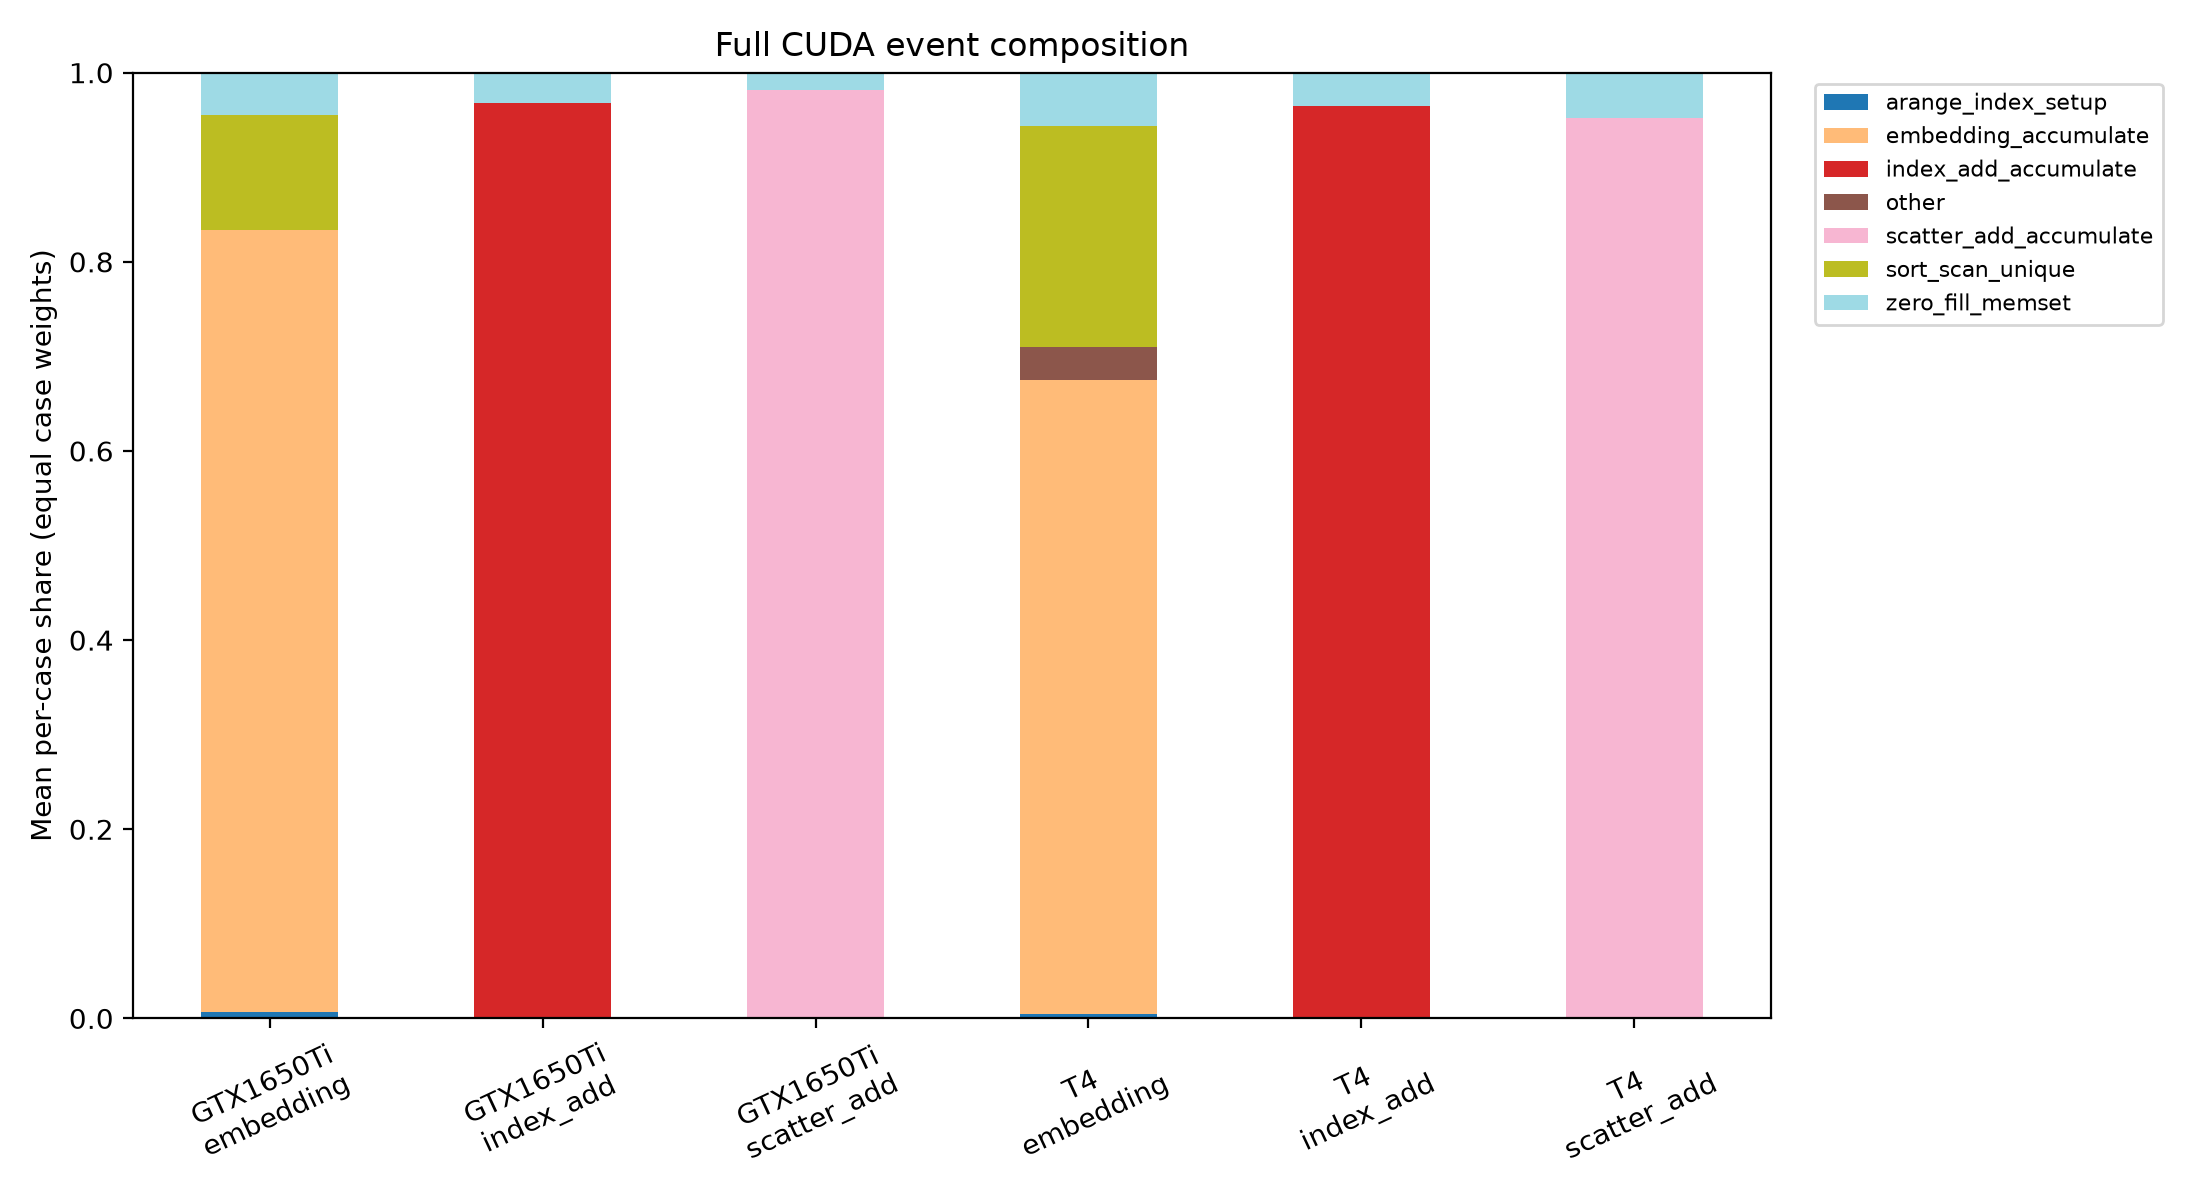
\includegraphics[width=0.95\linewidth]{figures/phase3_kernel_category_share.png}
\caption{Mean CUDA kernel-category share for the representative Phase 3 profiles. Category shares are computed from CUDA device events and summarize observed execution-path composition.}
\label{fig:phase3-kernel-category-share}
\end{figure*}

The mean category shares support the intended execution-path interpretation. In both environments, \texttt{index\_\allowbreak add} is dominated by the \texttt{index\_\allowbreak add\_\allowbreak accumulate} category, while \texttt{scatter\_\allowbreak add} is dominated by the \texttt{scatter\_\allowbreak add\_\allowbreak accumulate} category. The embedding backward path is dominated by \texttt{embedding\_\allowbreak accumulate}, but it also contains a non-trivial \texttt{sort\_\allowbreak scan\_\allowbreak unique} component. The \texttt{other} category remains below the selected control threshold, which reduces the risk that the main attribution is hiding a large unclassified portion of CUDA time.

\subsection{Case-Level Cross-Environment Comparison}

The Phase 3 case-level comparison links the representative profiling subset to both environments and to the broader Phase 2 grid. Table~\ref{tab:phase3-case-comparison} summarizes the raw case-level winners, margins, and winner-relation categories for the six representative cases.

% Source: ../sparse-gradient/phase3_comparison_v2/phase3_case_comparison.csv
\begin{table*}[t]
\centering
\fontsize{9}{11}\selectfont
\caption{Phase 3 case-level comparison across environments.}
\label{tab:phase3-case-comparison}
\setlength{\tabcolsep}{3pt}
\renewcommand{\arraystretch}{1.12}
\begin{tabular*}{\textwidth}{@{\extracolsep{\fill}}lrrrrl@{}}
\toprule
Case & Local winner & T4 winner & \shortstack{Local\\margin} & \shortstack{T4\\margin} & \shortstack{Winner\\relation} \\
\midrule
case01 & index\_add & scatter\_add & 1.670 & 1.022 & reversal near-tie \\
case02 & embedding & embedding & 2.631 & 1.706 & same decisive \\
case03 & embedding & scatter\_add & 1.116 & 1.186 & reversal decisive \\
case04 & index\_add & index\_add & 1.197 & 1.058 & same decisive \\
case05 & embedding & scatter\_add & 1.257 & 1.285 & reversal decisive \\
case06 & embedding & scatter\_add & 1.015 & 1.040 & reversal near-tie \\
\bottomrule
\end{tabular*}
\end{table*}

Two cases provide the strongest evidence of a cross-environment reversal. In case03, the GTX1650Ti stack selects \texttt{embedding} decisively, while the T4 stack selects \texttt{scatter\_\allowbreak add} decisively. In case05, the same pattern appears again: the GTX1650Ti stack selects \texttt{embedding}, whereas the T4 stack selects \texttt{scatter\_\allowbreak add}. Both cases pass the stronger clean-reversal gates in the comparison analysis: they are decisively separated, have clean GPU-busy proxy status, and use exact index pairing across environments.

Figure~\ref{fig:phase3-case-winner-comparison} visualizes the case-level winner comparison. The figure shows a mixture of agreement, near-ties, and decisive reversals within the diagnostic subset.

\begin{figure*}[t]
\centering
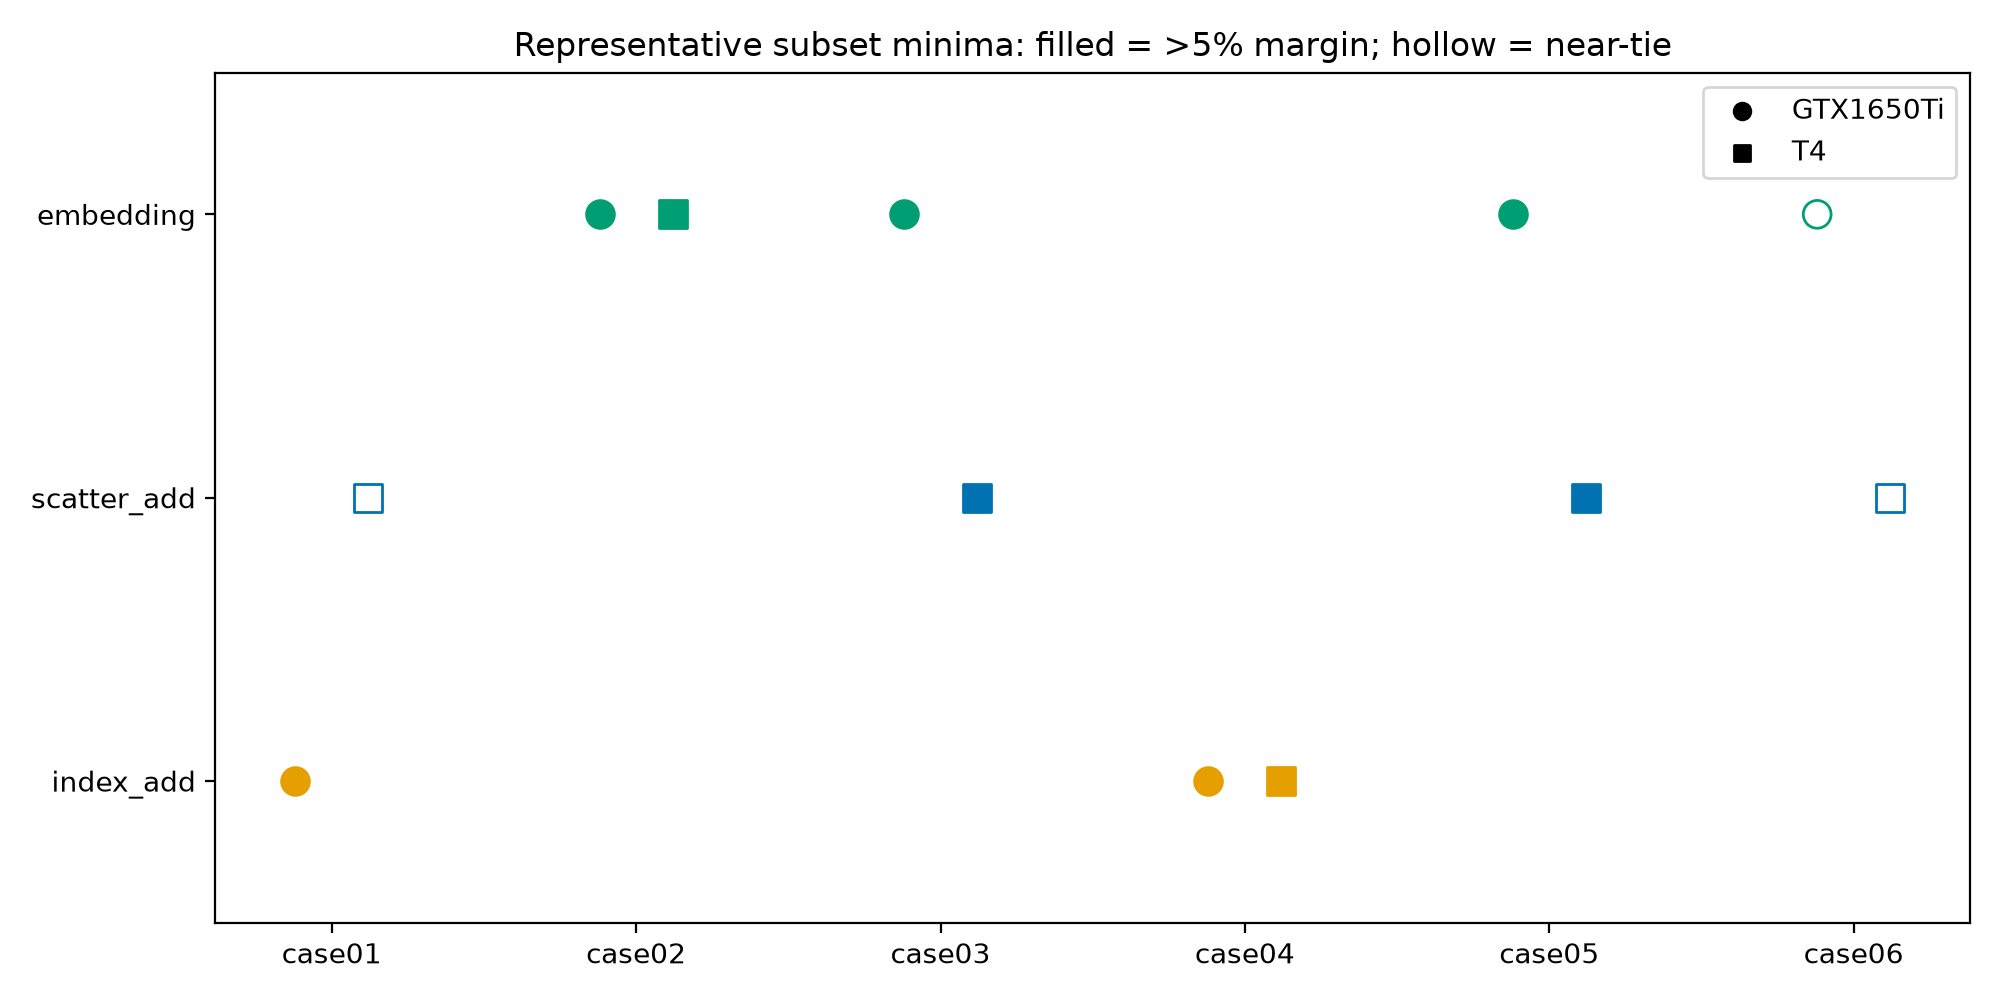
\includegraphics[width=0.95\linewidth]{figures/phase3_case_winner_comparison.png}
\caption{Representative Phase 3 winner comparison across environments. Filled markers indicate decisive practical-margin winners, while near-ties are interpreted as weak evidence.}
\label{fig:phase3-case-winner-comparison}
\end{figure*}

The remaining cases serve as controls or cautionary examples rather than strong claims of representativeness. In case02, both environments select \texttt{embedding} decisively. In case04, both environments select \texttt{index\_\allowbreak add} decisively, although the T4 \texttt{embedding} row has a host-overhead warning and therefore prevents a fully GPU-clean claim for that case. Cases case01 and case06 exhibit different raw winners across environments, but at least one side is a near-tie, so these cases are treated as weak evidence rather than decisive reversals.

The profiled cases were linked back to the broader Phase~2 grid. The strongest support comes from case03 and case05, where both the grid and profiling agree on a decisive reversal: the GTX1650Ti stack favors \texttt{Embedding.\allowbreak backward}, whereas the T4 stack favors \texttt{scatter\_\allowbreak add}. The remaining cases serve as controls or cautionary examples involving agreement, near-ties, or host-overhead warnings; the subset is diagnostic rather than statistically representative of the full grid.

The case-level evidence therefore reinforces the grid-level result without replacing it. Phase 2 establishes the broader matched-performance pattern, while Phase 3 explains selected cases in terms of execution-path differences. The combination of the two phases is stronger than either alone: the timing grid shows that the fastest API changes across environments, and the profiler shows that the compared APIs exercise distinct CUDA paths.

\subsection{CUDA Path Attribution}

Execution-path conclusions require consistent kernel-category attribution. Cross-environment reversal claims additionally require practical-margin separation, stable timing, exact index pairing, and no host-overhead warning.

% Evidence criteria retained in prose; diagnostic table excluded from the main flow.
% % Source: ../sparse-gradient/phase3_comparison_v2/phase3_claim_checks.csv
\begin{table}[tbp]
\centering
\fontsize{9}{11}\selectfont
\caption{Phase 3 claim-check status and source cautions.}
\label{tab:phase3-claim-checks}
\resizebox{\linewidth}{!}{%
\begin{tabular}{lp{0.12\linewidth}p{0.30\linewidth}p{0.36\linewidth}}
\toprule
Check & Passed & Supporting numbers & Caution \\
\midrule
index\_add\_path\_dominance & True & GTX1650Ti=0.9677; T4=0.9647 & Full-event CUDA category shares required. \\
scatter\_add\_path\_dominance & True & GTX1650Ti=0.9817; T4=0.9518 & Full-event CUDA category shares required. \\
embedding\_accumulation\_present & True & GTX1650Ti=0.8271; T4=0.6697 & Full-event CUDA category shares required. \\
embedding\_sort\_scan\_present & True & GTX1650Ti=0.1217; T4=0.2342 & Full-event CUDA category shares required. \\
other\_share\_controlled & True & T4/embedding=0.03467 & Unknown kernels substantial at mean other share $\geq 0.2$. \\
phase2\_environment\_difference\_present & True & GTX1650Ti=embedding; T4=scatter\_add; T4\_repeat=scatter\_add & Expected most-frequent decisive API required in the local run and both T4 runs. \\
representative\_reversals\_present & True & case03, case05 & Representative subset is illustrative, not statistical. \\
\bottomrule
\end{tabular}
}%
\end{table}

The \texttt{index\_\allowbreak add} path is dominated by the \texttt{index\_\allowbreak add\_\allowbreak accumulate} category in both environments, and the \texttt{scatter\_\allowbreak add} path is dominated by the \texttt{scatter\_\allowbreak add\_\allowbreak accumulate} category in both environments. This supports the claim that the two APIs dispatch to distinct CUDA reduction paths under the profiled workloads.

The embedding backward path contains a dominant accumulation component, but it also includes sorting, scanning, or uniqueness-related work. This distinguishes \texttt{Embedding.\allowbreak backward} from the direct \texttt{index\_\allowbreak add} and \texttt{scatter\_\allowbreak add} paths. The result is consistent with the interpretation that embedding backward is a specialized framework path rather than a simple alias for either direct accumulation API.

Within the profiled subset, case03 and case05 satisfy the strict evidence conditions: they are decisive reversals, they are not host-warning cases, they have stable timing evidence, and they use exact index pairing. These cases therefore support the paper-level statement that the relative cost of sparse-index accumulation paths can change with workload and software/hardware stack.

At the same time, the attribution remains conservative. The kernel categories are based on profiler event names and CUDA event durations, not on low-level hardware counters. They support execution-path attribution within the measured stacks; the hardware-causality limitations are detailed in Section~\ref{sec:methodology}.

% Standalone staged subsection; not inserted into the existing manuscript.
\subsection{Training-step proxy}
\label{sec:phase4-training-proxy}

To examine whether the sparse-index accumulation effects observed in isolated
measurements persist in a broader backpropagation-style setting, we introduced a
small synthetic training-step proxy. The proxy combines indexed lookup, grouped
mean pooling, a scalar linear prediction head, mean-squared error, and backward
propagation. The three variants use identical inputs, pooling, head, and loss.
The \texttt{embedding\_\allowbreak backward\_\allowbreak proxy} variant uses native dense Embedding
backward, whereas \texttt{index\_\allowbreak add\_\allowbreak proxy} and
\texttt{scatter\_\allowbreak add\_\allowbreak proxy} use custom autograd lookup nodes that allocate a
dense zero gradient and accumulate row gradients with the corresponding PyTorch
API.

Two timing scopes were recorded. The \texttt{proxy\_\allowbreak step} scope measures the
complete synthetic step: lookup, pooling, prediction, loss, and gradients for the
table, head, and bias. The \texttt{accumulation\_\allowbreak region} scope separately replays
backward through a retained lookup graph with fixed upstream gradients. This
second scope is diagnostic only: it includes autograd dispatch, dense gradient
allocation and zeroing, and accumulation, but it is not an exact decomposition of
the proxy step and must not be subtracted from total-step latency.

Each environment was evaluated with five seeds and 24 configurations per seed,
giving 120 seed--configuration observations per environment. The grid varied the
number of rows, number of references, embedding dimension, and index
distribution. All included runs completed successfully, and all configurations
and variants passed the recorded validation checks. As in the preceding
experiments, a variant is counted as a winner only when the runner-up median is
strictly more than 5\% slower; otherwise the observation is classified as a
practical tie.

Table~\ref{tab:phase4-winner-counts} and
Figure~\ref{fig:phase4-winner-counts} summarize the results. On the GTX1650Ti stack, \texttt{index\_\allowbreak add} dominated both scopes, winning 83 of 120
proxy-step observations and 98 of 120 accumulation-region observations. Native
Embedding won 10 observations in each scope, while the remaining cases were
classified as practical ties. On the T4 stack, practical ties dominated: 95 of
120 proxy-step observations and 78 of 120 accumulation-region observations. Among
the resolved T4 cases, the proxy step favored \texttt{scatter\_\allowbreak add} in 25
observations, while the accumulation-region diagnostic favored
\texttt{scatter\_\allowbreak add} in 39 observations and \texttt{index\_\allowbreak add} in three.

\begin{table*}[t]
\centering\fontsize{9}{11}\selectfont
\caption{Phase~4 winners under the strictly greater than 5\% practical-margin rule. Each environment contributes 120 seed--configuration observations. Region replay denotes the separate accumulation diagnostic scope.}
\label{tab:phase4-winner-counts}
\setlength{\tabcolsep}{3pt}
\renewcommand{\arraystretch}{1.12}
\begin{tabular*}{\textwidth}{@{\extracolsep{\fill}}llrrrrr@{}}
\toprule
Environment & Scope & \texttt{index\_add} & \texttt{scatter\_add} & Embedding & Tie & Total \\
\midrule
GTX1650Ti & Proxy step & 83 & 0 & 10 & 27 & 120 \\
GTX1650Ti & Region replay & 98 & 0 & 10 & 12 & 120 \\
T4 & Proxy step & 0 & 25 & 0 & 95 & 120 \\
T4 & Region replay & 3 & 39 & 0 & 78 & 120 \\
\bottomrule
\end{tabular*}
\end{table*}
% \begin{table}[tbp]
\centering\fontsize{9}{11}\selectfont
\caption{Descriptive Phase~4 outcomes by environment. The contrast is not attributed to GPU hardware alone because the software and host environments also differ.}
\label{tab:phase4-environment-comparison}
\setlength{\tabcolsep}{3pt}
\begin{tabularx}{\linewidth}{lXXX}
\toprule
Environment & Proxy-step outcome & Region-replay outcome & Interpretation \\
\midrule
GTX1650Ti & \texttt{index\_add}: 83/120 & \texttt{index\_add}: 98/120 & The local stack most often favors the custom \texttt{index\_add} path. \\
T4 & Tie: 95/120 & Tie: 78/120 & Most observations are unresolved; resolved cases mainly favor \texttt{scatter\_add}. \\
\bottomrule
\end{tabularx}
\end{table}

\begin{figure*}[t]
\centering
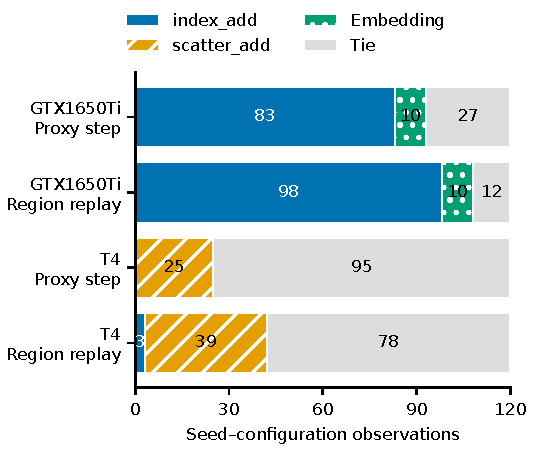
\includegraphics[width=0.60\linewidth]{figures/phase4_winner_counts_by_environment.pdf}
\caption{Phase~4 practical-margin winner counts across five seeds and 24
configurations per environment. Region replay denotes the separate accumulation
diagnostic scope. Ties are retained explicitly.}
\label{fig:phase4-winner-counts}
\end{figure*}

The proxy results reinforce the central conclusion that sparse-index accumulation
performance is conditional rather than universal. In the GTX1650Ti stack, the custom \texttt{index\_\allowbreak add} backward path was most often favored.
In the T4 stack, most observations were unresolved by the 5\% practical
margin rule, and the resolved cases mainly favored \texttt{scatter\_\allowbreak add}. This
contrast should not be interpreted as isolated GPU causality, because the two
environments also differ in PyTorch version, CUDA version, operating system, and
host settings. Instead, the result shows that rankings obtained from isolated
sparse-index accumulation measurements should not be transferred mechanically to
a training-step-like context without measurement.

This proxy remains deliberately limited. It does not measure convergence,
optimizer state, data loading, distributed training, or production-scale model
throughput. The manual variants use custom autograd lookup nodes, so the
comparison is at the API/path level and includes dispatch and graph overhead
rather than pure kernel speed. The \texttt{accumulation\_\allowbreak region} scope is a
diagnostic replay, not a decomposition of the proxy step.

\subsection{Practical-Margin Threshold Sensitivity}
\label{sec:threshold-sensitivity}

The primary analysis uses a strictly greater than 5\% practical-margin rule to avoid treating small median-latency differences as decisive API wins. To check whether the qualitative conclusions depend on this specific threshold, we recomputed winner counts using 2\%, 5\%, and 10\% thresholds from the saved per-variant median-latency artifacts. The fastest path is counted as a winner only when the runner-up median divided by the fastest median, minus one, exceeds the selected threshold. These sensitivity checks are descriptive robustness checks, not statistical tests; the main analysis retains the 5\% rule.

Table~\ref{tab:threshold-sensitivity-phase2} shows the Phase~2 sensitivity results over the same 162 matched configuration--draw observations per run. The recomputed 5\% counts reproduce the main analysis. Tie counts change by design: lower thresholds reduce their number, while higher thresholds increase it. The qualitative Phase~2 pattern remains across the tested thresholds: the GTX1650Ti stack most often favors \texttt{Embedding.\allowbreak backward}, while the T4 stack and its repeat run most often favor \texttt{scatter\_\allowbreak add}.

\begin{table*}[t]
\centering\fontsize{9}{11}\selectfont
\caption{Threshold sensitivity of Phase~2 winner counts. The main paper uses the strictly greater than 5\% practical-margin rule; 2\% and 10\% are reported only as sensitivity checks.}
\label{tab:threshold-sensitivity-phase2}
\setlength{\tabcolsep}{3pt}
\renewcommand{\arraystretch}{1.12}
\begin{tabular*}{\textwidth}{@{\extracolsep{\fill}}llrrrrr@{}}
\toprule
Environment & Threshold & \texttt{index\_add} & \texttt{scatter\_add} & Embedding & Tie & Total \\
\midrule
GTX1650Ti & 2\% & 61 & 0 & 99 & 2 & 162 \\
GTX1650Ti & 5\% & 60 & 0 & 96 & 6 & 162 \\
GTX1650Ti & 10\% & 52 & 0 & 91 & 19 & 162 \\
T4 & 2\% & 9 & 113 & 28 & 12 & 162 \\
T4 & 5\% & 5 & 92 & 25 & 40 & 162 \\
T4 & 10\% & 3 & 78 & 21 & 60 & 162 \\
T4 repeat & 2\% & 4 & 120 & 30 & 8 & 162 \\
T4 repeat & 5\% & 1 & 93 & 27 & 41 & 162 \\
T4 repeat & 10\% & 0 & 81 & 22 & 59 & 162 \\
\bottomrule
\end{tabular*}
\end{table*}


Table~\ref{tab:threshold-sensitivity-phase4} shows the corresponding Phase~4 sensitivity results for 120 seed--configuration observations per environment and scope. Its 5\% counts also reproduce the main analysis. On the GTX1650Ti stack, \texttt{index\_\allowbreak add} remains the most frequent resolved winner in both scopes across the tested thresholds. However, the proxy-step result becomes nearly balanced with ties at 10\% (58 \texttt{index\_\allowbreak add} wins versus 57 ties), while the accumulation replay remains more stable with 97 \texttt{index\_\allowbreak add} wins at the same threshold.

The T4 proxy step remains majority-tied at all three thresholds, with resolved cases mainly favoring \texttt{scatter\_\allowbreak add}. In the T4 accumulation replay, ties rise from 40/120 at 2\% to 78/120 at 5\% and 99/120 at 10\%; at 2\%, \texttt{scatter\_\allowbreak add} is the largest category with 58 wins. These results show that the qualitative workload-, scope-, and stack-dependent interpretation is stable, while the absolute balance between resolved outcomes and ties is threshold-sensitive.

\begin{table*}[t]
\centering\fontsize{9}{11}\selectfont
\caption{Threshold sensitivity of Phase~4 proxy winner counts. The main paper uses the strictly greater than 5\% practical-margin rule; 2\% and 10\% are reported only as sensitivity checks.}
\label{tab:threshold-sensitivity-phase4}
\setlength{\tabcolsep}{3pt}
\renewcommand{\arraystretch}{1.12}
\begin{tabular*}{\textwidth}{@{\extracolsep{\fill}}lllrrrrr@{}}
\toprule
Environment & Scope & Threshold & \texttt{index\_add} & \texttt{scatter\_add} & Embedding & Tie & Total \\
\midrule
GTX1650Ti & Proxy step & 2\% & 96 & 1 & 11 & 12 & 120 \\
GTX1650Ti & Proxy step & 5\% & 83 & 0 & 10 & 27 & 120 \\
GTX1650Ti & Proxy step & 10\% & 58 & 0 & 5 & 57 & 120 \\
GTX1650Ti & Region replay & 2\% & 106 & 0 & 11 & 3 & 120 \\
GTX1650Ti & Region replay & 5\% & 98 & 0 & 10 & 12 & 120 \\
GTX1650Ti & Region replay & 10\% & 97 & 0 & 10 & 13 & 120 \\
T4 & Proxy step & 2\% & 2 & 42 & 0 & 76 & 120 \\
T4 & Proxy step & 5\% & 0 & 25 & 0 & 95 & 120 \\
T4 & Proxy step & 10\% & 0 & 18 & 0 & 102 & 120 \\
T4 & Region replay & 2\% & 22 & 58 & 0 & 40 & 120 \\
T4 & Region replay & 5\% & 3 & 39 & 0 & 78 & 120 \\
T4 & Region replay & 10\% & 0 & 21 & 0 & 99 & 120 \\
\bottomrule
\end{tabular*}
\end{table*}


As an additional descriptive stability check, we computed bootstrap intervals for selected aggregate winner shares from the saved 5\% winner classifications. These intervals are not hypothesis tests and do not support inference to all possible workloads, GPUs, or software versions. They summarize resampling variability conditional on the saved observations.

In Phase~2, the dominant-share intervals preserve the same qualitative pattern. The GTX1650Ti \texttt{Embedding.\allowbreak backward} share is 59.3\%, with a 95\% descriptive interval of 51.9--66.7\%. The \texttt{scatter\_\allowbreak add} shares are 56.8\% on T4 and 57.4\% on the T4 repeat, with intervals of 49.4--64.2\% and 50.0--64.8\%, respectively. In Phase~4, observation-level intervals support the GTX1650Ti \texttt{index\_\allowbreak add} tendency and the T4 tie-heavy interpretation, while configuration-cluster intervals are wider. For example, the GTX1650Ti proxy-step \texttt{index\_\allowbreak add} share is 69.2\%, with an observation-level interval of 60.8--77.5\% and a configuration-cluster interval of 50.8--85.8\%. The wider cluster interval reinforces that the proxy should be interpreted as a controlled descriptive study rather than a population-level statistical estimate.

\subsection{Result-Level Discussion}

The combined results answer the central question of the study: standard PyTorch CUDA APIs that express related sparse-index accumulation behavior do not necessarily have interchangeable performance characteristics during backpropagation-style workloads. In the matched Phase 2 grid, the GTX1650Ti stack most often favors the embedding backward path, whereas the T4 stack and its repeat run most often favor \texttt{scatter\_\allowbreak add}. In the representative Phase 3 profiles, the strongest reversal cases show the same pattern at the case level: GTX1650Ti execution favors \texttt{embedding}, while T4 execution favors \texttt{scatter\_\allowbreak add}.

The results also show why the difference should not be reduced to a simple API ranking. Some representative cases agree across environments, some differ only as near-ties, and two cases provide strong decisive reversals. This mixed behavior indicates that the best operation depends on workload shape, index distribution, duplicate structure, and the software/hardware stack. A recommendation such as ``always use \texttt{scatter\_\allowbreak add}'' or ``always use \texttt{Embedding.\allowbreak backward}'' would not be supported by the evidence.

The execution-path attribution provides a practical explanation for this behavior. Although the operations represent related accumulation-style computations, they dispatch to different CUDA paths. \texttt{index\_\allowbreak add} and \texttt{scatter\_\allowbreak add} use different direct accumulation kernels, while \texttt{Embedding.\allowbreak backward} uses a multi-kernel path that includes embedding-specific accumulation and sorting or segmentation-related work. These differences create opportunities for the relative cost of the APIs to change when the workload or execution stack changes.

For practitioners, the results suggest that sparse-gradient accumulation paths in AI training should not be selected purely from high-level API semantics. When sparse-index accumulation is a relevant part of the backward pass, especially in embedding-heavy models, recommender workloads, or other skewed-index settings, the actual execution path and target environment can materially affect performance. Microbenchmarking and profiler inspection remain useful tools for identifying which API path is most appropriate for a specific workload and deployment stack.

Finally, the results define the boundary of the present evidence. The study characterizes controlled sparse-index accumulation workloads and representative profiler cases; it does not measure full model training throughput, convergence behavior, distributed execution, or custom CUDA alternatives. Therefore, the contribution is best understood as a controlled characterization of PyTorch CUDA sparse-index gradient accumulation paths during backpropagation-style computation, rather than as a complete benchmark of AI training systems.